\documentclass[11pt,a4paper]{article}

% ================================================================ packages
\usepackage[T1]{fontenc}
\usepackage[utf8]{inputenc}
\usepackage{newtxtext,newtxmath}
\usepackage[margin=2.4cm]{geometry}
\usepackage{amsmath,amssymb}
\usepackage{graphicx}
\usepackage{booktabs}
\usepackage{adjustbox}
\usepackage{xcolor}
\usepackage{xspace}
\usepackage[font=small,labelfont=bf]{caption}
\usepackage[numbers,sort&compress]{natbib}
\usepackage[colorlinks=true,linkcolor=violet,citecolor=blue!60!black,urlcolor=blue!60!black]{hyperref}
\usepackage{microtype}
\usepackage{fancyhdr}

% arXiv-preprint look (same running head as the widely used arxiv.sty template)
\pagestyle{fancy}
\fancyhf{}
\renewcommand{\headrulewidth}{0.4pt}
\fancyhead[C]{\small\scshape A Preprint, \today}
\fancyfoot[C]{\thepage}
\fancypagestyle{plain}{\fancyhf{}\renewcommand{\headrulewidth}{0pt}\fancyfoot[C]{\thepage}}
\setlength{\headheight}{14pt}

\graphicspath{{figures/}}
\newcommand{\ie}{i.e.\@\xspace}
\newcommand{\eg}{e.g.\@\xspace}

% ================================================================ title
\title{\bfseries Label Noise Moves the Threshold, Not the Ranking:\\
Classical Baselines versus Evidential Uncertainty\\ for Pneumonia Detection with Uncertain Labels}

\author{
  \begin{adjustbox}{max width=\textwidth}
  \begin{tabular}{@{}c@{\hspace{3em}}c@{}}
    FOFACK ALEMDJOU Henri Jo\"el\textsuperscript{*} & ELOUNDOU NGOUMA Thomas Christian \\
    {\small 22P231} & {\small 22P294} \\[6pt]
    WATON JEUTA Ivana & WAFO TEGUO Vitric Val\`ere \\
    {\small 24P763} & {\small 22P446} \\[6pt]
    ZUCHUON KOUGANG Nathanael Michel & AYISSI NGONO Odile Marie Ange \\
    {\small 22P218} & {\small 24P764}
  \end{tabular}
  \end{adjustbox}\\[10pt]
  \small Department of Computer Engineering\\
  \small National Advanced School of Engineering of Yaound\'e (NASEY)\\
  \small University of Yaound\'e I, Cameroon\\[4pt]
  \small \textsuperscript{*}Corresponding author
}
\date{}

\begin{document}
\maketitle

\begin{abstract}
Medical image labels are often uncertain, yet classical classifiers treat them as exact. We study this gap on
PneumoniaMNIST. Nine classical models, including a from-scratch logistic regression trained by stochastic gradient
ascent, boosted trees and kernel SVMs, are tuned on validation data and stressed by flipping 0--40\% of the
minority-class training labels; an evidential CNN is compared with an identical softmax CNN. Three findings emerge.
First, asymmetric label noise mainly shifts the decision threshold: specificity collapses from about 0.6 to 0.2--0.3
while ROC-AUC stays within 0.92--0.95. Second, stronger regularisation consistently hurts, whereas re-selecting the
threshold on a small clean set keeps accuracy between 0.85 and 0.89 up to 40\% noise. Third, the evidential model
matches softmax accuracy and is better calibrated under noise (expected calibration error 0.13 versus 0.21 at 20\%
noise), but its uncertainty does not reliably improve out-of-distribution detection. All results are reproducible
from public notebooks and MLflow runs.
\end{abstract}

\noindent\textbf{Keywords:} medical image classification $\cdot$ label noise $\cdot$ uncertain labels $\cdot$
evidential deep learning $\cdot$ Dempster--Shafer theory $\cdot$ calibration $\cdot$ precision--recall $\cdot$ MLOps

% ======================================================================
\section{Introduction}
% ======================================================================
Supervised medical image classifiers are trained on labels that are themselves uncertain. Radiologists disagree on
ambiguous findings, labels mined automatically from free-text reports inherit the hedging of those reports (CheXpert
explicitly marks such observations as \emph{uncertain}~\cite{irvin2019chexpert}), and annotation errors are
unavoidable at scale~\cite{karimi2020deep}. A model fitted as if these labels were exact may memorise the
noise~\cite{zhang2017understanding} and, more insidiously, returns a confident probability for every input, including
inputs it has no evidence about.

Classical machine learning offers two generic answers to label noise: \emph{regularisation} (a larger penalty in
logistic regression or support vector machines, shallower trees, slower boosting) and careful \emph{evaluation} on
metrics that remain informative under class imbalance~\cite{saito2015precision}. Neither, however, gives the model a
way to say ``I do not know''. Evidential deep learning (EDL)~\cite{sensoy2018evidential} does: grounded in
Dempster--Shafer theory~\cite{dempster1967upper,shafer1976mathematical} and subjective logic~\cite{josang2016subjective},
it lets a network output a Dirichlet distribution whose total strength measures the amount of evidence, and turns the
lack of evidence into an explicit uncertainty mass. Evidential uncertainty has been used on chest radiographs to
reject unreliable cases and to flag likely annotation errors~\cite{ghesu2019quantifying,ghesu2021quantifying}.

This report studies, on a deliberately lightweight but realistic benchmark (PneumoniaMNIST~\cite{yang2023medmnist}),
how far classical robustness tools go against label uncertainty, and what an evidential model adds. Our contributions are:
\begin{enumerate}
  \item a complete, validation-tuned evaluation of nine classical classifiers, including a from-scratch logistic
        regression trained by stochastic gradient ascent (SGA), with bootstrap confidence intervals and a controlled
        study of why precision--recall curves must replace ROC curves when the disease is rare;
  \item a factorial label-noise study (clean/noisy $\times$ baseline/regularised/recalibrated, 0--40\% flipped
        minority labels, repeated seeds) showing that asymmetric label noise mainly \emph{moves the decision threshold}
        while leaving the ranking almost intact, and that stronger regularisation does not help;
  \item a PyTorch implementation of an evidential CNN compared with an identical softmax CNN, evaluated not only on
        accuracy but on what the uncertainty is good for: referring doubtful cases, detecting out-of-distribution
        images and spotting flipped training labels;
  \item a reproducible MLOps pipeline (MLflow tracking, model registry) and public notebooks generating every number,
        table and figure of this report.
\end{enumerate}

% ======================================================================
\section{Related Work}
% ======================================================================
\paragraph{Classical classification and regularisation.}
Logistic regression trained by stochastic gradient methods~\cite{robbins1951stochastic,bottou2010large}, naive
Bayes~\cite{domingos1997optimality}, nearest neighbours~\cite{beyer1999nearest}, decision trees~\cite{breiman1984classification},
boosting~\cite{freund1997decision,friedman2001greedy} and (kernel) support vector machines~\cite{cortes1995support,scholkopf2002learning}
remain strong baselines on small medical datasets. Their capacity is controlled by explicit regularisation: the
inverse penalty $C$, tree depth and leaf size, or the learning rate and number of boosting rounds.

\paragraph{Learning with noisy labels.}
Label noise has been surveyed extensively~\cite{frenay2014classification,song2022learning}, including in medical
imaging~\cite{karimi2020deep}. Remedies include loss correction under a known noise
model~\cite{natarajan2013learning}, noise-robust losses~\cite{ghosh2017robust,zhang2018generalized}, and
identification of mislabelled examples, \eg by confident learning~\cite{northcutt2021confident}. Deep networks can fit
arbitrary labels~\cite{zhang2017understanding}, so their behaviour under noise depends heavily on training choices.

\paragraph{Uncertainty quantification.}
Bayesian approximations such as Monte-Carlo dropout~\cite{gal2016dropout} and deep ensembles~\cite{lakshminarayanan2017simple}
estimate uncertainty from several forward passes. Prior networks~\cite{malinin2018prior} and EDL~\cite{sensoy2018evidential}
instead predict the parameters of a Dirichlet distribution in a single pass; see~\cite{ulmer2023prior} for a survey.
Uncertainty is typically assessed through calibration~\cite{guo2017calibration}, misclassification and
out-of-distribution (OOD) detection~\cite{hendrycks2017baseline}, and selective prediction~\cite{geifman2017selective}.
In chest radiography, Ghesu \emph{et al.}~\cite{ghesu2019quantifying,ghesu2021quantifying} showed that evidential
uncertainty supports rejecting ambiguous cases and identifying label noise.

% ======================================================================
\section{Methodology}
% ======================================================================
\subsection{Data and preprocessing}
PneumoniaMNIST~\cite{yang2023medmnist} contains paediatric chest radiographs~\cite{kermany2018identifying} resized to
$28\times28$ grey-level pixels, with official patient-disjoint splits of 4\,708 (train), 524 (validation) and 624
(test) images. The task is binary: $y=1$ (pneumonia, the positive class) versus $y=0$ (normal). Normal images are the
minority class (25.8\% of the training set); the prevalence of pneumonia drops from 74.2\% (train and validation) to
62.5\% (test), a realistic acquisition shift (Fig.~\ref{fig:samples}). For classical models each image is flattened
to $x\in[0,1]^{784}$ and standardised with training statistics. The dataset has no missing values; a simulated 5\%
missing-completely-at-random pixel mask, imputed inside the pipeline, lowered validation accuracy of logistic regression
only from 0.958 to 0.952 (mean imputation). \textbf{All hyper-parameters are selected on the validation split}; the test
split is used once, for reporting.

\subsection{Classical models}
\paragraph{Logistic regression by SGA.} We maximise the $\ell_2$-penalised log-likelihood with per-sample updates
\begin{equation}
  \theta \leftarrow \theta + \alpha_t\big[(y_i - \sigma(\theta^\top x_i + b))\,x_i - \lambda\theta\big],\qquad
  \alpha_t = \frac{\alpha_0}{1+\kappa t},
\end{equation}
with $\alpha_0=0.01$, $\lambda=0.01$, $\kappa=10^{-4}$, 30 epochs. Each update costs $O(m)$ instead of $O(nm)$ for
batch gradient ascent; on a 200\,000-sample synthetic problem SGA came within 0.005 of the best validation
log-likelihood after 0.69 passes over the data, against 34 passes for batch gradient ascent (Fig.~\ref{fig:sga}).
The multiclass (softmax) extension reaches 67.7\% test accuracy on the 11-class OrganCMNIST, on par with scikit-learn's
multinomial solver (67.4\%). The sigmoid output is read as $P(y=1\mid x)$, \ie a log-odds model whose calibration we
check with a reliability diagram (Fig.~\ref{fig:logreg}). We also report the L-BFGS solution of
scikit-learn~\cite{pedregosa2011scikit} ($C=10^{-3}$).

\paragraph{Other models.} Gaussian naive Bayes, whose conditional-independence assumption is strongly violated by
neighbouring pixels (correlation $\approx0.92$) but which trains in a single $O(nm)$ pass; $K$-nearest neighbours
($K=7$, Euclidean), which degrades much less with dimension than distance concentration on uniform data would suggest,
because radiographs lie on a low-dimensional manifold (Fig.~\ref{fig:knn}); CART with Gini impurity
(depth 13, $\geq5$ samples per leaf), whose fitting time we verified to grow linearly in $n$, $m$ and depth
(Fig.~\ref{fig:tree}); AdaBoost with depth-2 trees (186 rounds, learning rate 0.5); histogram gradient boosting
(54 rounds, 15 leaves, learning rate 0.1, $\ell_2=1$); a soft-margin linear SVM (hinge loss, $C=3.2\times10^{-3}$);
and an RBF-kernel SVM ($C=3$, $\gamma=10^{-3}$) selected on a $4\times4$ validation grid. The role of $C$ on the
margin and the number of support vectors, and the implicit feature map of kernels, are illustrated in
Figs.~\ref{fig:svm} and~\ref{fig:kernel}.

\subsection{Label-noise model and robust variants}
Following the assignment, uncertain labels are simulated by flipping a fraction $\rho$ of the \emph{minority-class}
training labels (normal $\to$ pneumonia), \ie with the class-conditional transition
$P(\tilde y=1\mid y=0)=\rho$, $P(\tilde y=0\mid y=1)=0$. We use $\rho=5\%$ (61 of 1\,214 normal images, 10 random
draws) and a sweep $\rho\in\{0,5,10,20,30,40\}\%$ (5 draws). Validation and test labels are never corrupted. The three
best models on validation within the families named by the assignment (boosted trees, kernel SVM and regularised
logistic regression) are retrained in three configurations:
(i)~\emph{baseline} (validation-selected hyper-parameters);
(ii)~\emph{robust}: stronger regularisation ($C/10$ for SVM and logistic regression; 7 leaves, half learning rate,
$\ell_2=10$ and $\geq50$ samples per leaf for boosting);
(iii)~\emph{recalibrated}: the baseline model whose decision threshold is re-selected to maximise balanced accuracy on
the clean validation set (a small trusted set, no parameter re-estimation).

\subsection{Evidential CNN}
Both deep models share the same CNN (three $3\times3$ convolution blocks with batch normalisation, 16/32/64 channels,
global average pooling, dropout 0.3, linear layer; 23\,650 parameters) and training recipe (Adam, learning rate
$10^{-3}$, weight decay $10^{-4}$, batch size 128, 15 epochs, 3 seeds), implemented in PyTorch~\cite{paszke2019pytorch};
only the output layer and loss differ.
The \textbf{softmax} model is trained with cross-entropy. The \textbf{evidential} model~\cite{sensoy2018evidential}
maps logits $z$ to non-negative evidence $e_k=\mathrm{softplus}(z_k)$ and Dirichlet parameters $\alpha_k=e_k+1$. With
$S=\sum_k\alpha_k$ and $K=2$ classes, subjective logic~\cite{josang2016subjective} gives belief masses $b_k=e_k/S$ and an
uncertainty (ignorance) mass $u=K/S$ with $\sum_k b_k+u=1$, and the expected class probability is $\hat p_k=\alpha_k/S$.
The loss is the Bayes risk of the cross-entropy under the Dirichlet plus an annealed Kullback--Leibler term that removes
evidence not supported by the label:
\begin{equation}
  \mathcal L_i=\sum_{k}y_{ik}\big(\psi(S_i)-\psi(\alpha_{ik})\big)
  +\lambda_t\,\mathrm{KL}\!\left(\mathrm{Dir}(p\mid\tilde\alpha_i)\,\big\|\,\mathrm{Dir}(p\mid\mathbf 1)\right),\quad
  \tilde\alpha_i=y_i+(1-y_i)\odot\alpha_i,\quad \lambda_t=\min(1,t/10),
\end{equation}
where $\psi$ is the digamma function and $t$ the epoch. Unlike the softmax output, the Dirichlet can express ``no
evidence'' ($S\to K$, $u\to1$) separately from ``balanced evidence'' ($\hat p\approx0.5$ with small $u$).

\subsection{Evaluation protocol}
We report accuracy, precision, recall (sensitivity), specificity, F1, ROC-AUC and average precision (AP, area under the
precision--recall curve), with 95\% bootstrap confidence intervals (1\,000 resamples of the test set). Calibration is
measured by the expected calibration error (ECE, 15 bins)~\cite{guo2017calibration}. Uncertainty scores (normalised
predictive entropy for the softmax model, $u$ for EDL) are assessed by the AUROC for (a)~separating misclassified from
correct test predictions, (b)~separating the PneumoniaMNIST test set from OOD images of other modalities (BreastMNIST
ultrasound and OrganCMNIST CT~\cite{yang2023medmnist}), and (c)~retrieving flipped training labels. Every run of the
noise study is tracked with MLflow~\cite{zaharia2018accelerating} (hyper-parameters, metrics, serialised model with its
input signature), and the final model is versioned in the MLflow model registry.

% ======================================================================
\section{Experiments and Results}
% ======================================================================
\subsection{Classical baselines on clean labels}
Table~\ref{tab:clean} and Fig.~\ref{fig:rocpr} summarise the nine classical models trained on clean labels. The kernel
SVM ranks patients best (ROC-AUC 0.947, AP 0.961), the linear SVM has the best accuracy and F1 (0.864 and 0.900), and
our from-scratch SGA logistic regression (accuracy 0.851, ROC-AUC 0.927) is on par with the L-BFGS solution. The 95\%
bootstrap intervals of F1 are wide and overlap substantially (\eg $[0.859, 0.905]$ for logistic regression versus
$[0.880, 0.920]$ for the linear SVM): on 624 test images, the differences among the leading models are within the
sampling uncertainty. The single tree is clearly the weakest ranker (ROC-AUC 0.747), and boosting repairs
this (0.931 for AdaBoost, 0.938 for gradient boosting; Fig.~\ref{fig:boosting}). All models share one weakness: a recall
of 0.90--0.99 but a specificity of only 0.57--0.73. Validation accuracies were much higher (up to 0.973 for the RBF-SVM),
because the threshold learned at a 74\% pneumonia prevalence is too aggressive for the 62.5\% prevalence of the test set.
Decision boundaries on a 2-D PCA projection (Fig.~\ref{fig:boundaries}) illustrate the inductive biases: a single
straight line with smoothly varying probabilities for logistic regression, axis-aligned staircases with piecewise-constant
probabilities for the tree, and a smooth curved frontier for the RBF-SVM.

\begin{figure}[t]
  \centering
  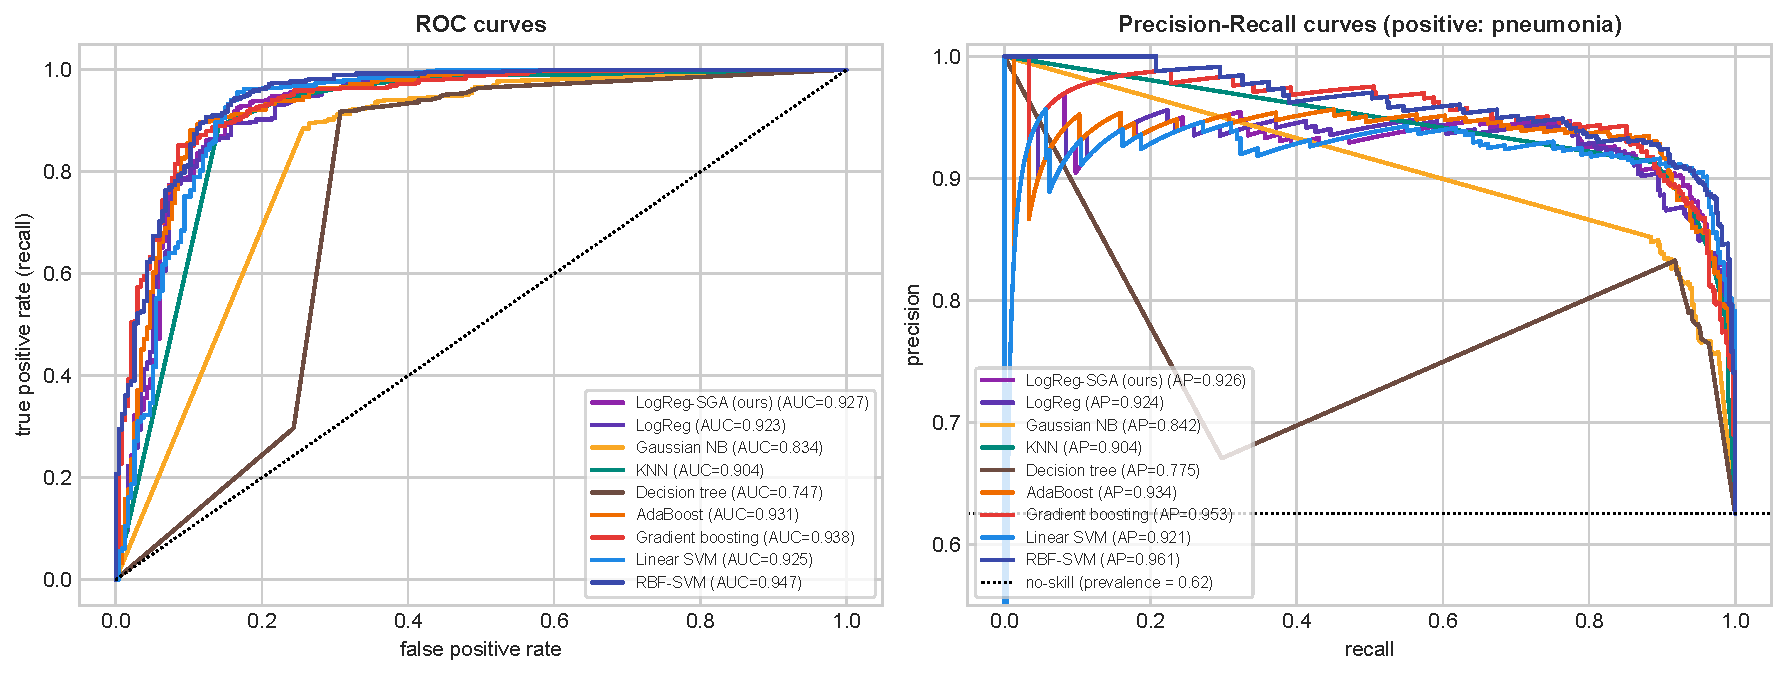
\includegraphics[width=\linewidth]{fig_roc_pr}
  \caption{ROC (left) and precision--recall (right) curves of the classical models on the clean test set
           (positive class: pneumonia). The dotted line of the PR plot is the no-skill level, \ie the prevalence.}
  \label{fig:rocpr}
\end{figure}

\begin{table}[t]
\centering
\small
\caption{Test performance of all classical models trained on clean labels (positive class: pneumonia; 95\% bootstrap confidence interval for F1). Best value per column in bold.}
\label{tab:clean}
\begin{adjustbox}{max width=\textwidth}
\begin{tabular}{lccccccc}
\toprule
Model & Acc. & Prec. & Recall & Spec. & F1 [95\% CI] & ROC-AUC & AP \\
\midrule
LogReg-SGA (ours) & 0.851 & 0.814 & 0.987 & 0.624 & 0.892 [0.870, 0.913] & 0.927 & 0.926 \\
LogReg & 0.837 & 0.800 & 0.985 & 0.590 & 0.883 [0.859, 0.905] & 0.923 & 0.924 \\
Gaussian NB & 0.833 & \textbf{0.847} & 0.895 & \textbf{0.731} & 0.870 [0.846, 0.894] & 0.834 & 0.842 \\
KNN & 0.830 & 0.793 & 0.985 & 0.573 & 0.879 [0.856, 0.902] & 0.904 & 0.904 \\
Decision tree & 0.804 & 0.790 & 0.936 & 0.585 & 0.857 [0.831, 0.881] & 0.747 & 0.775 \\
AdaBoost & 0.840 & 0.806 & 0.979 & 0.607 & 0.884 [0.861, 0.906] & 0.931 & 0.934 \\
Gradient boosting & 0.830 & 0.800 & 0.972 & 0.594 & 0.877 [0.853, 0.900] & 0.938 & 0.953 \\
Linear SVM & \textbf{0.864} & 0.831 & 0.982 & 0.667 & 0.900 [0.880, 0.920] & 0.925 & 0.921 \\
RBF-SVM & 0.857 & 0.818 & \textbf{0.992} & 0.632 & 0.897 [0.874, 0.919] & \textbf{0.947} & \textbf{0.961} \\
\bottomrule
\end{tabular}
\end{adjustbox}
\end{table}


\subsection{Why precision--recall instead of ROC under imbalance}
Pneumonia is the \emph{majority} class of PneumoniaMNIST, whereas screening typically targets a rare disease. Keeping
the RBF-SVM fixed, we subsampled the pneumonia cases of the test set to vary the prevalence from 50\% to 5\%
(200 draws each, Fig.~\ref{fig:prevalence}). The ROC-AUC does not move (0.947--0.949), while the average precision falls
from 0.938 to 0.544$\pm$0.107. The false-positive rate divides false alarms by the (large) number of healthy patients
and therefore hides them when the disease is rare; precision compares them with the true detections, which is what a
clinician experiences. The PR curve is thus the honest summary for imbalanced medical data~\cite{saito2015precision,davis2006relationship}.

\begin{figure}[t]
  \centering
  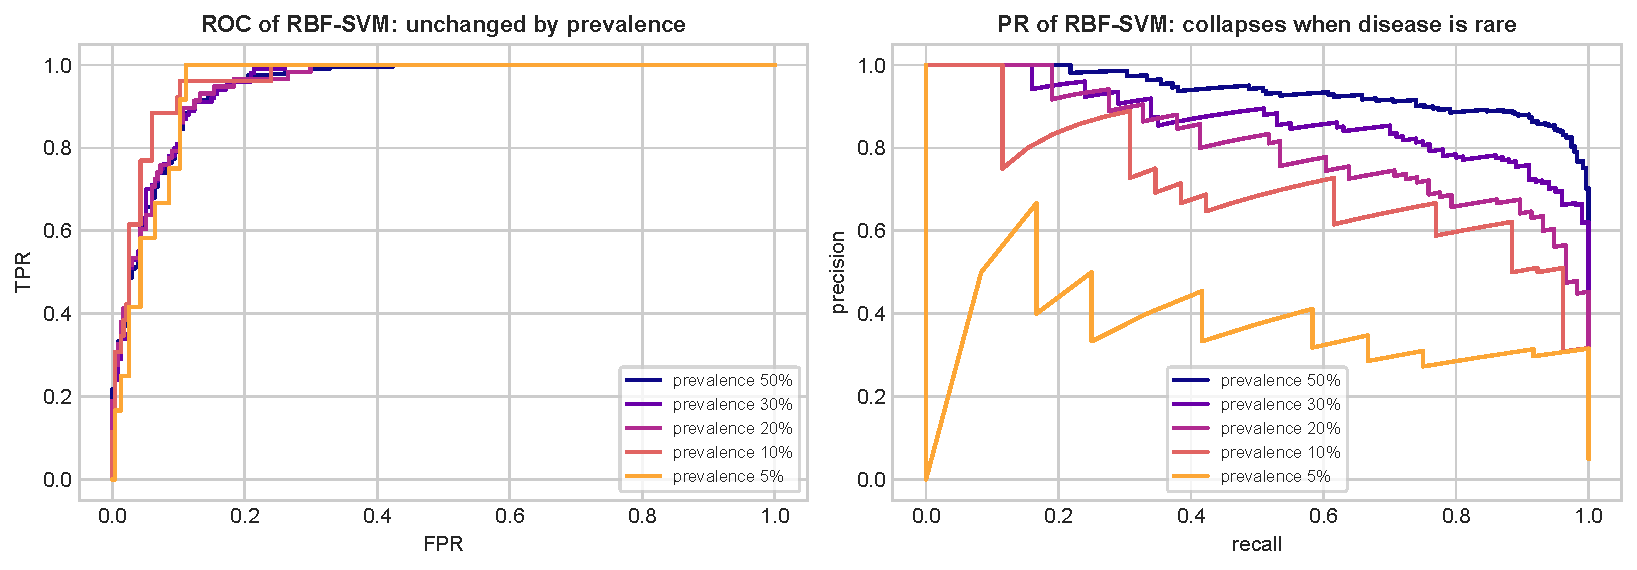
\includegraphics[width=\linewidth]{fig_prevalence}
  \caption{Same classifier (RBF-SVM), same scores: ROC curves are invariant to the prevalence of the positive class,
           precision--recall curves collapse when the disease becomes rare.}
  \label{fig:prevalence}
\end{figure}

\subsection{Robustness of classical models to label noise}
With 5\% of the normal training labels flipped (Table~\ref{tab:noise5}), baseline models lose about one point of
accuracy and 2--4 points of specificity, while their ROC-AUC is unchanged; F1, dominated by the majority class, barely
moves. The sweep of Fig.~\ref{fig:noise_classical} reveals the mechanism. Up to 40\% of flipped minority labels, the
specificity of the baselines collapses from about 0.6 to 0.19--0.32 and their accuracy falls to 0.70--0.74, yet the
ROC-AUC stays within 0.92--0.95: \textbf{asymmetric label noise moves the decision threshold rather than the ranking}.
The models still order patients correctly, but they have learned an inflated pneumonia prevalence. Consistently,
\textbf{stronger regularisation does not help}: the regularised variants are worse than the baselines at every noise
level, because a more constrained model leans more on the (corrupted) class prior. Conversely, simply re-selecting the
threshold on the small clean validation set keeps the accuracy of all three models between 0.85 and 0.89 from 0\% to
40\% noise. This remedy requires a trusted labelled subset and does not tell \emph{which} training labels are wrong.

\begin{table}[t]
\centering
\small
\caption{Robustness to flipping 5\% of the minority-class (normal) training labels. \emph{baseline}: hyper-parameters selected on validation; \emph{robust}: stronger regularisation; \emph{recalibrated}: baseline with the decision threshold re-selected on the clean validation set. Clean: single run; noisy: mean$\pm$std over 10 random flips. $\Delta$ = noisy $-$ clean (the test set is always clean).}
\label{tab:noise5}
\begin{adjustbox}{max width=\textwidth}
\begin{tabular}{llccccccccc}
\toprule
Model & Config. & Acc. clean & Acc. noisy & $\Delta$Acc. & Spec. clean & Spec. noisy & $\Delta$Spec. & AUC clean & AUC noisy & $\Delta$AUC \\
\midrule
Gradient boosting & baseline & 0.830 & 0.825$\pm$0.005 & -0.006 & 0.594 & 0.560$\pm$0.013 & -0.034 & 0.938 & 0.940$\pm$0.003 & +0.002 \\
Gradient boosting & recalibrated & 0.838 & 0.867$\pm$0.011 & +0.029 & 0.624 & 0.721$\pm$0.056 & +0.097 & 0.938 & 0.940$\pm$0.003 & +0.002 \\
Gradient boosting & robust & 0.824 & 0.806$\pm$0.006 & -0.018 & 0.573 & 0.521$\pm$0.016 & -0.052 & 0.932 & 0.930$\pm$0.002 & -0.001 \\
RBF-SVM & baseline & 0.857 & 0.849$\pm$0.004 & -0.008 & 0.632 & 0.609$\pm$0.011 & -0.023 & 0.947 & 0.947$\pm$0.002 & -0.001 \\
RBF-SVM & recalibrated & 0.872 & 0.875$\pm$0.016 & +0.004 & 0.671 & 0.692$\pm$0.055 & +0.021 & 0.947 & 0.947$\pm$0.002 & -0.001 \\
RBF-SVM & robust & 0.841 & 0.833$\pm$0.004 & -0.008 & 0.598 & 0.570$\pm$0.011 & -0.029 & 0.946 & 0.946$\pm$0.001 & -0.000 \\
LogReg & baseline & 0.837 & 0.826$\pm$0.003 & -0.011 & 0.590 & 0.550$\pm$0.008 & -0.039 & 0.923 & 0.923$\pm$0.001 & -0.000 \\
LogReg & recalibrated & 0.865 & 0.869$\pm$0.004 & +0.003 & 0.722 & 0.725$\pm$0.015 & +0.003 & 0.923 & 0.923$\pm$0.001 & -0.000 \\
LogReg & robust & 0.822 & 0.802$\pm$0.002 & -0.020 & 0.551 & 0.494$\pm$0.004 & -0.058 & 0.920 & 0.919$\pm$0.000 & -0.000 \\
\bottomrule
\end{tabular}
\end{adjustbox}
\end{table}


\begin{figure}[t]
  \centering
  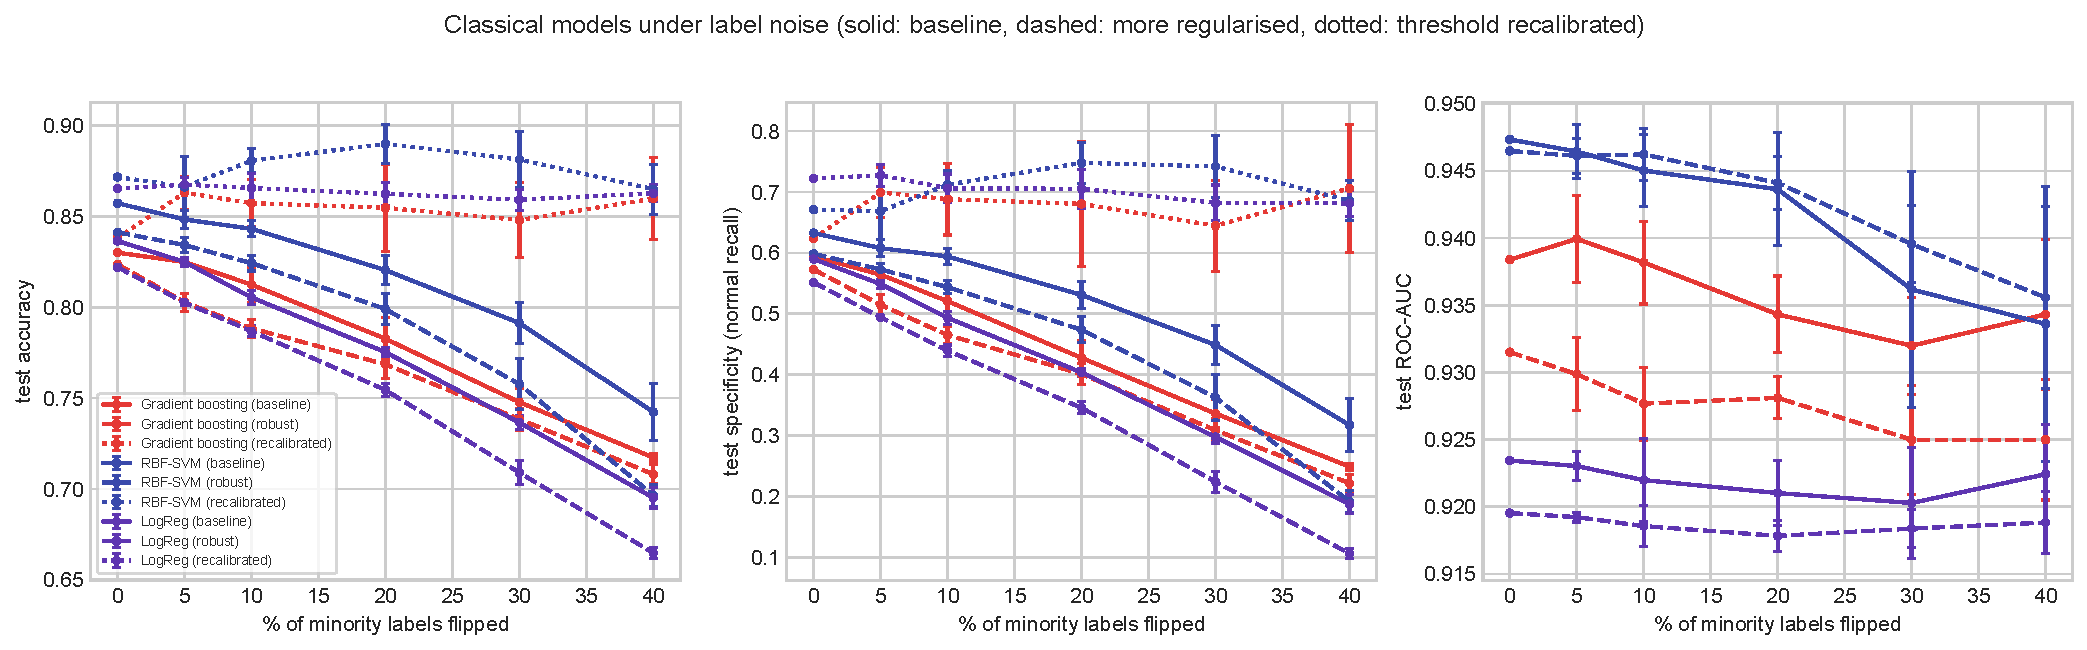
\includegraphics[width=\linewidth]{fig_noise_sweep_classical}
  \caption{Test accuracy, specificity and ROC-AUC of the three selected classical models as an increasing fraction of
           minority (normal) training labels is flipped (mean$\pm$std over 5 draws). Solid: baseline; dashed: stronger
           regularisation; dotted: baseline with the decision threshold recalibrated on the clean validation set.}
  \label{fig:noise_classical}
\end{figure}

\subsection{Evidential versus softmax CNN}
Table~\ref{tab:edl} and Fig.~\ref{fig:noise_all} compare the two CNNs with the best classical model. At the default
threshold of 0.5, both CNNs are \emph{less} accurate than the RBF-SVM (0.779$\pm$0.067 for softmax and 0.761$\pm$0.084
for EDL on clean labels, versus 0.857) and vary strongly across seeds, although they rank patients as well
(ROC-AUC 0.94--0.96). Small CNNs over-fit the training prevalence even more than the classical models: their
specificity is low and unstable. Once the threshold is re-selected on the clean validation set, all models converge to
an accuracy of 0.86--0.87 on clean labels. At equal architecture, the evidential head neither improves nor degrades
classification: at every noise level, the mean accuracies of the softmax and EDL models differ by at most 0.03, well
within their seed-to-seed spread (Fig.~\ref{fig:noise_all}). The evidential model is, however, consistently \textbf{better calibrated}: its expected calibration error
is lower at all six noise levels, and the gap widens under noise (0.144 versus 0.174 on clean labels, 0.126 versus 0.206
at 20\% and 0.187 versus 0.241 at 40\% flipped labels). The KL term, which removes evidence not supported by the labels,
prevents the over-confidence that cross-entropy induces on contradictory examples.

\begin{table}[t]
\centering
\small
\caption{Clean test performance after training with flipped minority labels (mean$\pm$std over seeds: 5 for the classical model, 3 for the CNNs). \emph{recal.}: decision threshold re-selected on the clean validation set. ECE: expected calibration error (lower is better).}
\label{tab:edl}
\begin{adjustbox}{max width=\textwidth}
\begin{tabular}{llcccccc}
\toprule
Noise & Model & Acc. & Spec. & ROC-AUC & Acc. (recal.) & Spec. (recal.) & ECE \\
\midrule
0\% & RBF-SVM (classical) & 0.857 & 0.632 & 0.947 & 0.872 & 0.671 & -- \\
0\% & CNN softmax & 0.779$\pm$0.067 & 0.419$\pm$0.187 & 0.946$\pm$0.001 & 0.869$\pm$0.010 & 0.682$\pm$0.012 & 0.174$\pm$0.080 \\
0\% & CNN EDL & 0.761$\pm$0.084 & 0.377$\pm$0.250 & 0.940$\pm$0.014 & 0.860$\pm$0.011 & 0.661$\pm$0.040 & 0.144$\pm$0.075 \\
5\% & RBF-SVM (classical) & 0.848$\pm$0.005 & 0.608$\pm$0.014 & 0.946$\pm$0.002 & 0.866$\pm$0.017 & 0.668$\pm$0.060 & -- \\
5\% & CNN softmax & 0.810$\pm$0.055 & 0.504$\pm$0.158 & 0.946$\pm$0.011 & 0.856$\pm$0.025 & 0.634$\pm$0.073 & 0.129$\pm$0.054 \\
5\% & CNN EDL & 0.798$\pm$0.096 & 0.486$\pm$0.298 & 0.950$\pm$0.025 & 0.862$\pm$0.038 & 0.660$\pm$0.114 & 0.128$\pm$0.045 \\
20\% & RBF-SVM (classical) & 0.821$\pm$0.008 & 0.531$\pm$0.022 & 0.944$\pm$0.004 & 0.890$\pm$0.011 & 0.748$\pm$0.034 & -- \\
20\% & CNN softmax & 0.722$\pm$0.049 & 0.259$\pm$0.129 & 0.950$\pm$0.013 & 0.855$\pm$0.012 & 0.658$\pm$0.045 & 0.206$\pm$0.058 \\
20\% & CNN EDL & 0.755$\pm$0.053 & 0.349$\pm$0.146 & 0.949$\pm$0.021 & 0.863$\pm$0.037 & 0.681$\pm$0.126 & 0.126$\pm$0.050 \\
\bottomrule
\end{tabular}
\end{adjustbox}
\end{table}


\begin{figure}[t]
  \centering
  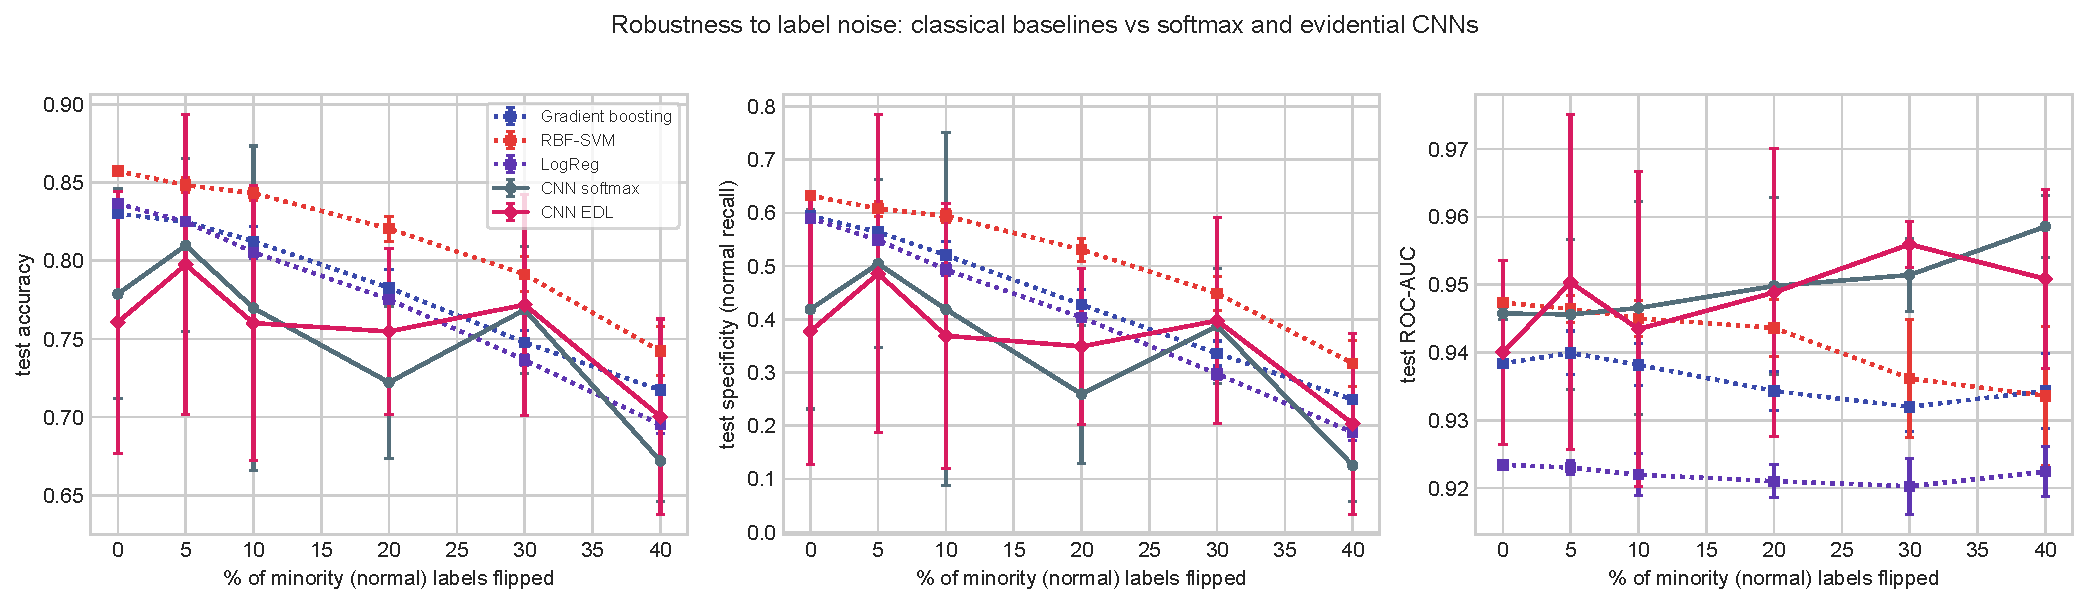
\includegraphics[width=\linewidth]{fig_noise_sweep_all}
  \caption{Classical baselines (dotted, 5 draws) versus softmax and evidential CNNs (solid, 3 seeds) under increasing
           minority-label noise, at the default decision threshold.}
  \label{fig:noise_all}
\end{figure}

\subsection{What is the evidential uncertainty good for?}
Table~\ref{tab:uncertainty} and Fig.~\ref{fig:uncertainty} evaluate the uncertainty itself.
\emph{Referral of doubtful cases.} Both uncertainty scores separate misclassified from correct test predictions with an
AUROC of about 0.80--0.84, without a consistent winner. For the seed shown in Fig.~\ref{fig:uncertainty} (left), the
evidential model retains a higher accuracy at almost every referral rate, in particular when trained with 20\% noise;
with three seeds, this observation should be confirmed on more runs.
\emph{Flipped training labels.} With 20\% of the normal labels flipped, the uncertainty ranks flipped training images
above the others with an AUROC of 0.88 for both models, and the disagreement between the evidential prediction and the
given label reaches 0.924$\pm$0.060 (0.899 for softmax). Fig.~\ref{fig:uncertainty} (right) qualifies this result: the
flipped images receive a high $u$ \emph{because they are normal radiographs}: the whole contested class becomes
uncertain, rather than each flipped example being singled out among its normal peers. The signal is therefore useful to
direct re-annotation towards the affected class rather than to pinpoint individual errors.
\emph{Out-of-distribution images.} The evidential $u$ does not consistently outperform the softmax entropy: it is worse
on ultrasound images (0.763 versus 0.814 on clean labels), comparable on CT images, and better on CT only after training
with noisy labels (0.847 versus 0.795). Fig.~\ref{fig:dirichlet} illustrates what the Dirichlet output adds: on the test
image where the evidential model is most undecided, softmax predicts pneumonia with probability 0.83 whereas EDL returns
a symmetric $\mathrm{Beta}(2.9, 2.9)$ with $u=0.35$; on an ultrasound image, softmax answers 0.56, EDL a flat density with
$u=0.46$, that is, ``I do not know'' rather than ``slightly more likely pneumonia''.

\begin{table}[t]
\centering
\small
\caption{AUROC of uncertainty scores (mean$\pm$std over 3 seeds) for detecting misclassified test images, out-of-distribution images (BreastMNIST ultrasound, OrganCMNIST CT) and flipped training labels. \emph{Disagr.}: $1-\hat p(\text{given label})$.}
\label{tab:uncertainty}
\begin{adjustbox}{max width=\textwidth}
\begin{tabular}{llccccc}
\toprule
Train noise & Model (uncertainty) & Misclass. & OOD breast & OOD CT & Flipped ($u$) & Flipped (disagr.) \\
\midrule
0\% & CNN EDL ($u=K/S$) & 0.830$\pm$0.006 & 0.763$\pm$0.029 & 0.650$\pm$0.213 & n/a & n/a \\
0\% & CNN softmax (entropy) & 0.822$\pm$0.016 & 0.814$\pm$0.009 & 0.675$\pm$0.065 & n/a & n/a \\
20\% & CNN EDL ($u=K/S$) & 0.801$\pm$0.030 & 0.753$\pm$0.110 & 0.847$\pm$0.026 & 0.882$\pm$0.012 & 0.924$\pm$0.060 \\
20\% & CNN softmax (entropy) & 0.836$\pm$0.051 & 0.829$\pm$0.043 & 0.795$\pm$0.031 & 0.885$\pm$0.017 & 0.899$\pm$0.058 \\
\bottomrule
\end{tabular}
\end{adjustbox}
\end{table}


\begin{figure}[t]
  \centering
  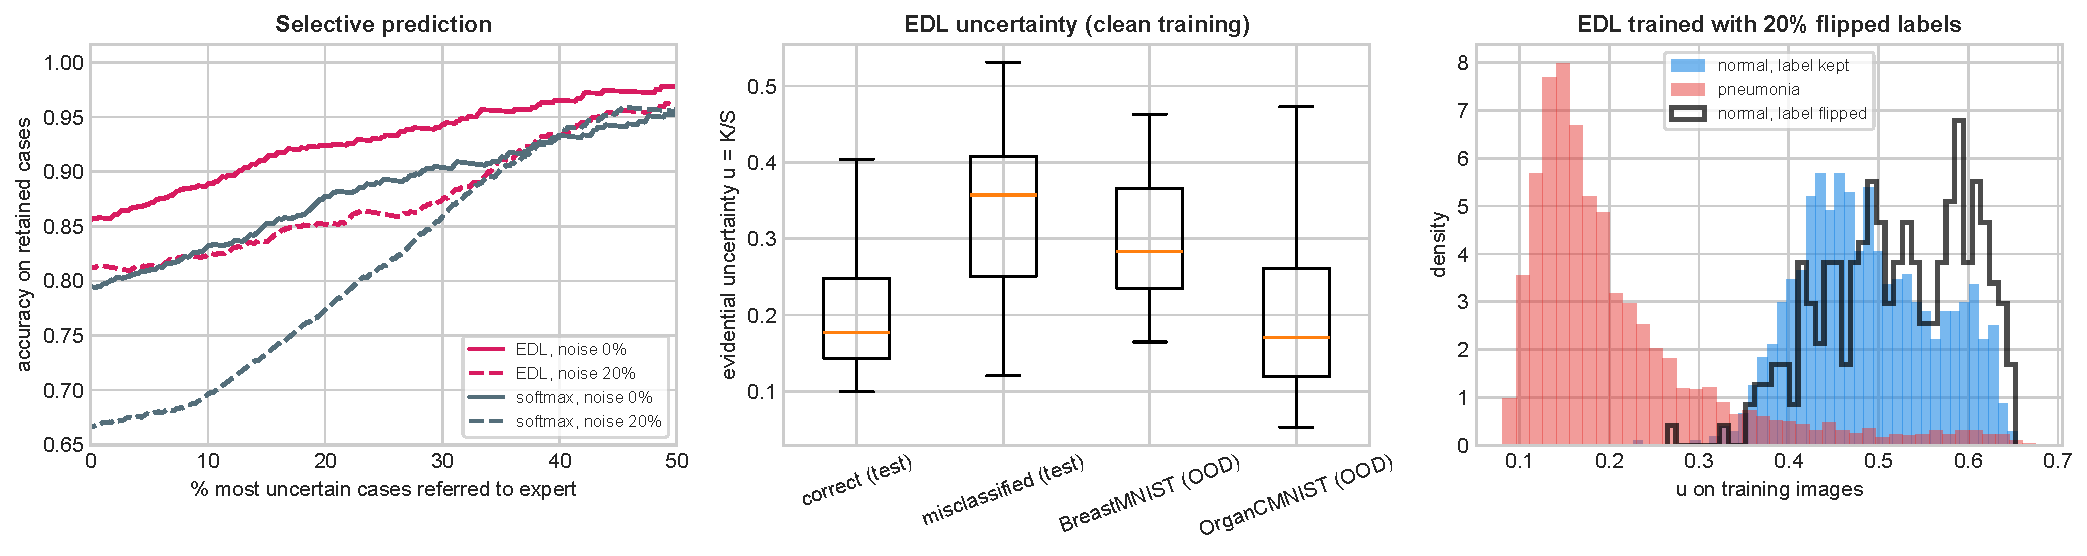
\includegraphics[width=\linewidth]{fig_uncertainty}
  \caption{Left: selective prediction, \ie accuracy on the retained cases when the most uncertain test images are referred
           to an expert (seed 0). Centre: evidential uncertainty of correct, misclassified and out-of-distribution
           images (clean training). Right: evidential uncertainty on the training images after flipping 20\% of the
           normal labels.}
  \label{fig:uncertainty}
\end{figure}

\begin{figure}[t]
  \centering
  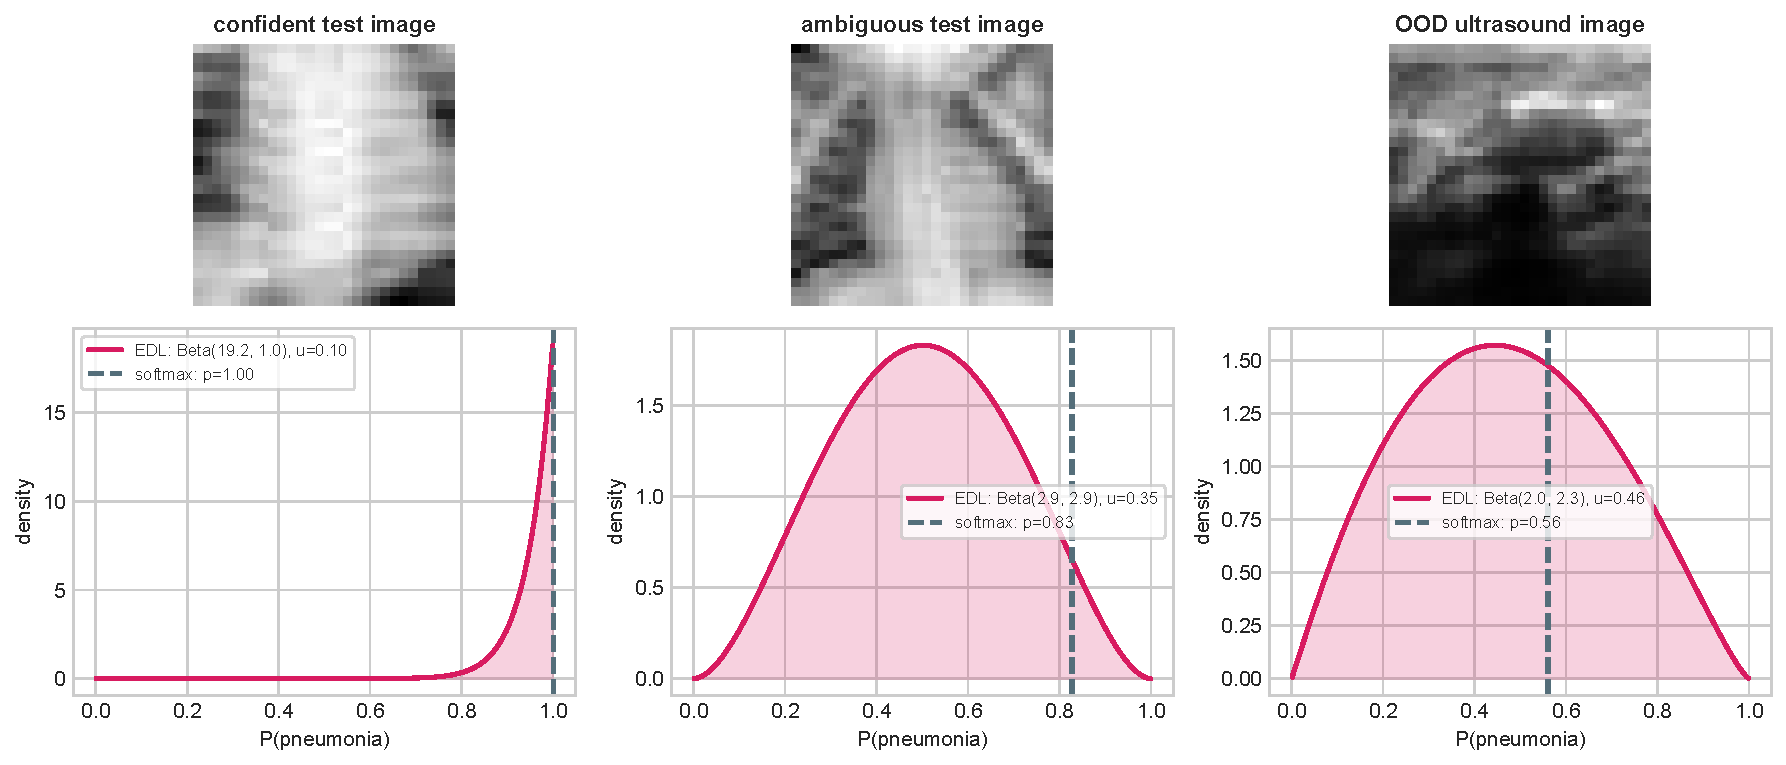
\includegraphics[width=0.92\linewidth]{fig_dirichlet}
  \caption{Dirichlet (here Beta, $K=2$) outputs of the evidential CNN for a confident test image, the test image on
           which it is most undecided and an out-of-distribution ultrasound image, against the softmax point
           prediction of the CNN with the same architecture.}
  \label{fig:dirichlet}
\end{figure}

% ======================================================================
\section{Discussion and Limitations}
% ======================================================================
Our experiments separate two effects that are often conflated under the term ``robustness to label noise''. For
class-conditional noise on the minority class, the dominant effect is a \emph{prior shift}: the learned class prior is
inflated, the ranking is preserved, and the damage is undone by recalibrating a single threshold on trusted data.
Regularisation, by contrast, addresses \emph{memorisation}, which is not the failure mode here and even worsens the
prior shift. Evidential learning brings a third, orthogonal benefit: calibrated confidence and an explicit ignorance
mass, which make the model's failures more visible rather than less frequent.

These conclusions have limits. Images are $28\times28$, which favours classical models and limits the CNNs; the noise
is synthetic and class-conditional, whereas real annotation errors depend on the image; a single dataset with a marked
train/test prevalence shift is used; the CNNs were trained with three seeds on CPU and show a large variance; and the
threshold recalibration assumes a small clean validation set, which is a realistic but not free resource in clinical
practice. Out-of-distribution detection was evaluated on two other MedMNIST modalities only.

% ======================================================================
\section{Conclusion and Future Work}
% ======================================================================
On PneumoniaMNIST, flipping minority-class labels mainly moves the decision threshold of classical classifiers while
leaving their ranking intact. Stronger regularisation does not help, but recalibrating the threshold on a small clean set
neutralises most of the damage. An evidential CNN classifies as well as its softmax twin, is better calibrated under
noise and expresses ignorance explicitly, although its uncertainty is not a reliable out-of-distribution detector in our
setting. Towards a full evidential pipeline, we plan to (i)~use the evidential uncertainty to re-weight or relabel
suspicious training examples rather than only to report it; (ii)~exploit multiple annotators and the explicit
\emph{uncertain} labels of CheXpert~\cite{irvin2019chexpert} at full resolution, where deep models have a real advantage;
(iii)~combine EDL with prior-shift correction and post-hoc calibration; and (iv)~compare it with deep ensembles and
Monte-Carlo dropout~\cite{lakshminarayanan2017simple,gal2016dropout} on equal computational budgets.

\section*{Acknowledgements}
This work was carried out as Practical Work~4 of the Machine Learning course of the Department of Computer Engineering,
National Advanced School of Engineering of Yaound\'e (NASEY), University of Yaound\'e~I, under the supervision of Dr.~Louis Fippo Fitime, Claude Tinku and Kerolle Sonfack.

\section*{Code and data availability}
PneumoniaMNIST, OrganCMNIST and BreastMNIST are publicly available from MedMNIST~\cite{yang2023medmnist}. The four
notebooks, the shared module and the MLflow configuration that produce every number, table and figure of this report
are provided with it; all hyper-parameters were selected on the validation split and all random seeds are fixed.

\bibliographystyle{plainnat}
\bibliography{references}

% ======================================================================
\appendix
\section{Supplementary figures (Phases I and II)}
% ======================================================================
\begin{figure}[h]
  \centering
  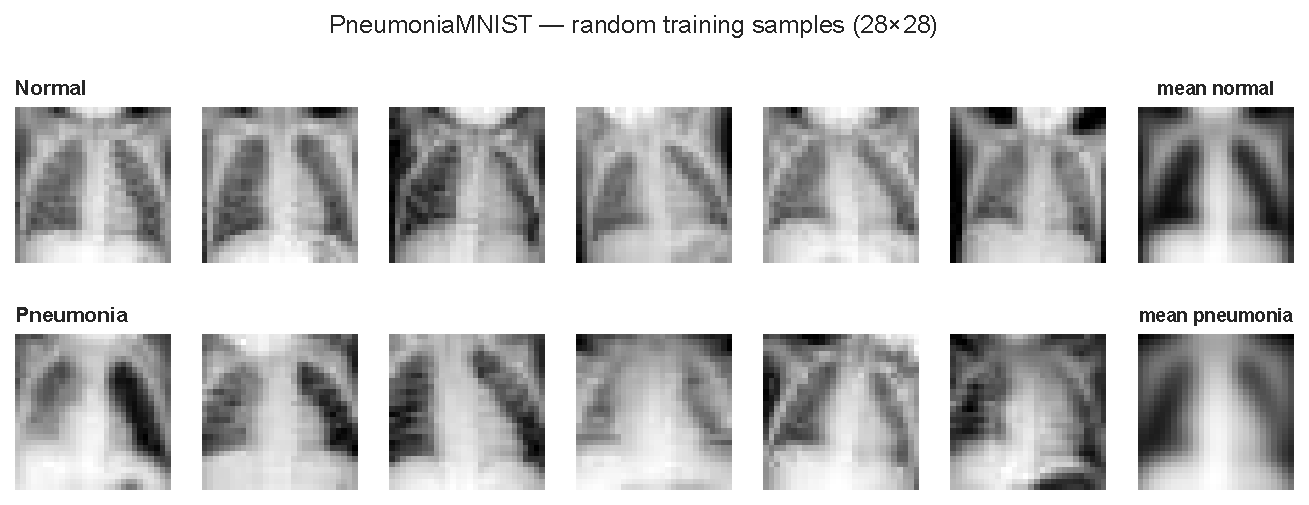
\includegraphics[width=0.85\linewidth]{fig_samples}
  \caption{Random PneumoniaMNIST training images and class-mean images.}
  \label{fig:samples}
\end{figure}

\begin{figure}[h]
  \centering
  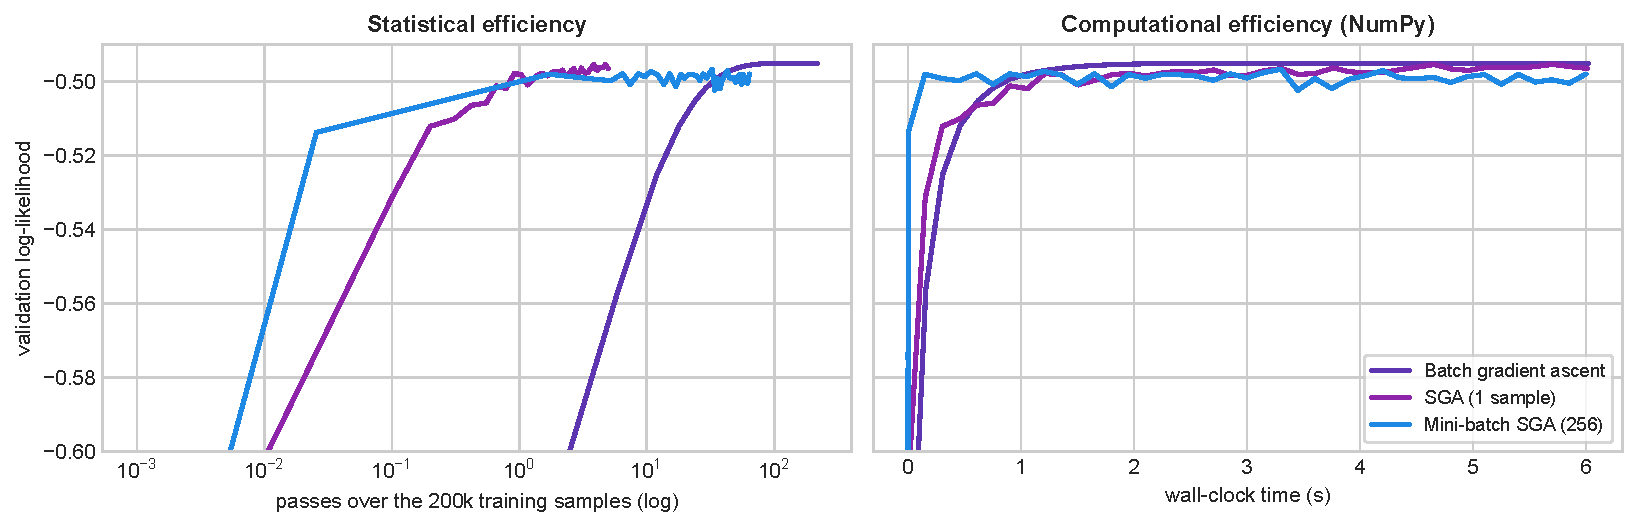
\includegraphics[width=\linewidth]{fig_sga_scaling}
  \caption{Logistic regression on 200\,000 synthetic samples. Left: validation log-likelihood against the number of
           passes over the data: stochastic updates need a fraction of one pass, batch gradient ascent tens of passes.
           Right: wall-clock time: the per-sample Python loop pays an interpreter overhead, mini-batch SGA combines both
           advantages.}
  \label{fig:sga}
\end{figure}

\begin{figure}[h]
  \centering
  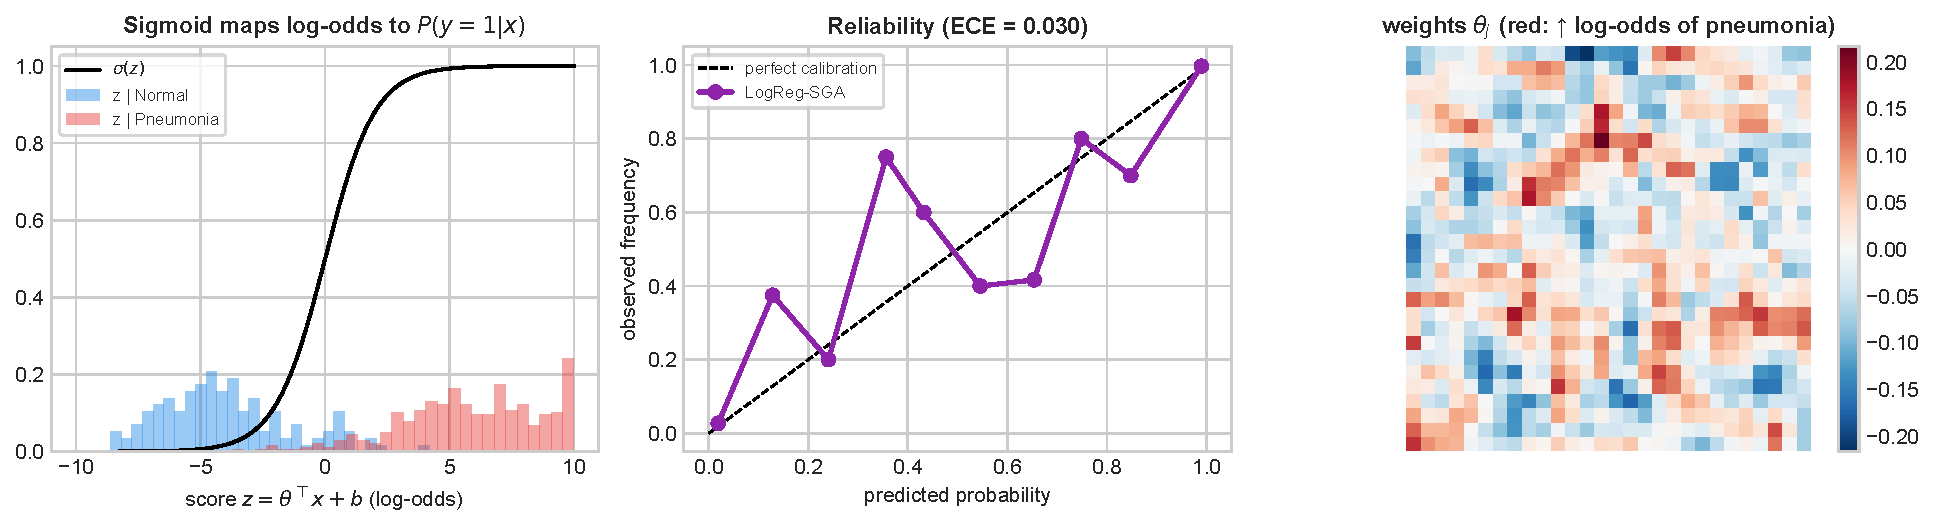
\includegraphics[width=\linewidth]{fig_logreg_proba}
  \caption{Probabilistic reading of the sigmoid (SGA logistic regression, validation set): log-odds per class,
           reliability diagram, and weights $\theta_j$ displayed as an image.}
  \label{fig:logreg}
\end{figure}

\begin{figure}[h]
  \centering
  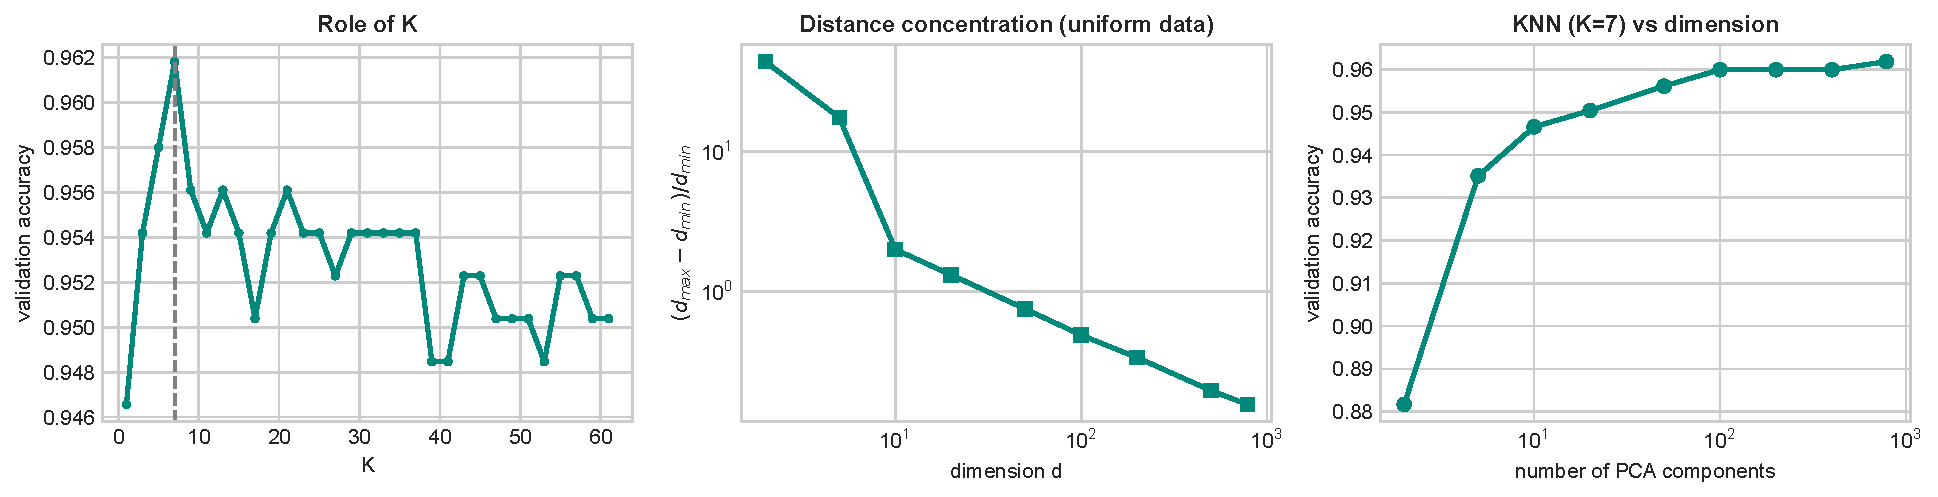
\includegraphics[width=\linewidth]{fig_knn}
  \caption{$K$-nearest neighbours: validation accuracy against $K$; distance concentration on uniform data; accuracy
           against the number of PCA components. Radiographs lie on a low-dimensional manifold, so KNN degrades much less
           than the uniform case suggests.}
  \label{fig:knn}
\end{figure}

\begin{figure}[h]
  \centering
  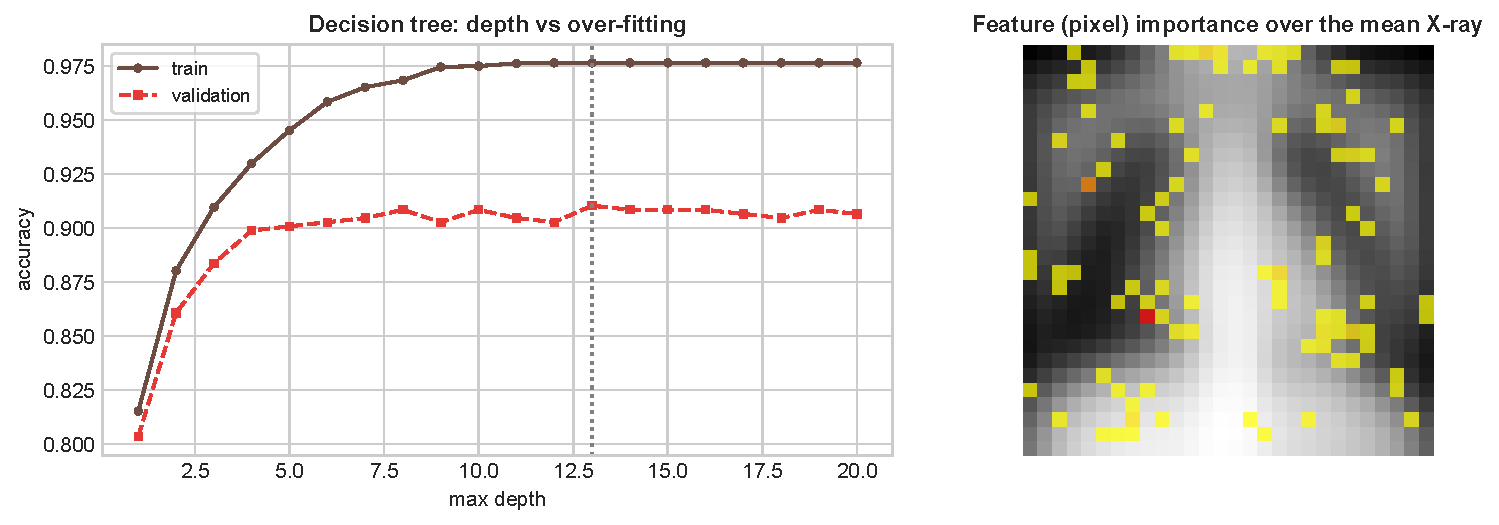
\includegraphics[width=0.9\linewidth]{fig_tree}\\[4pt]
  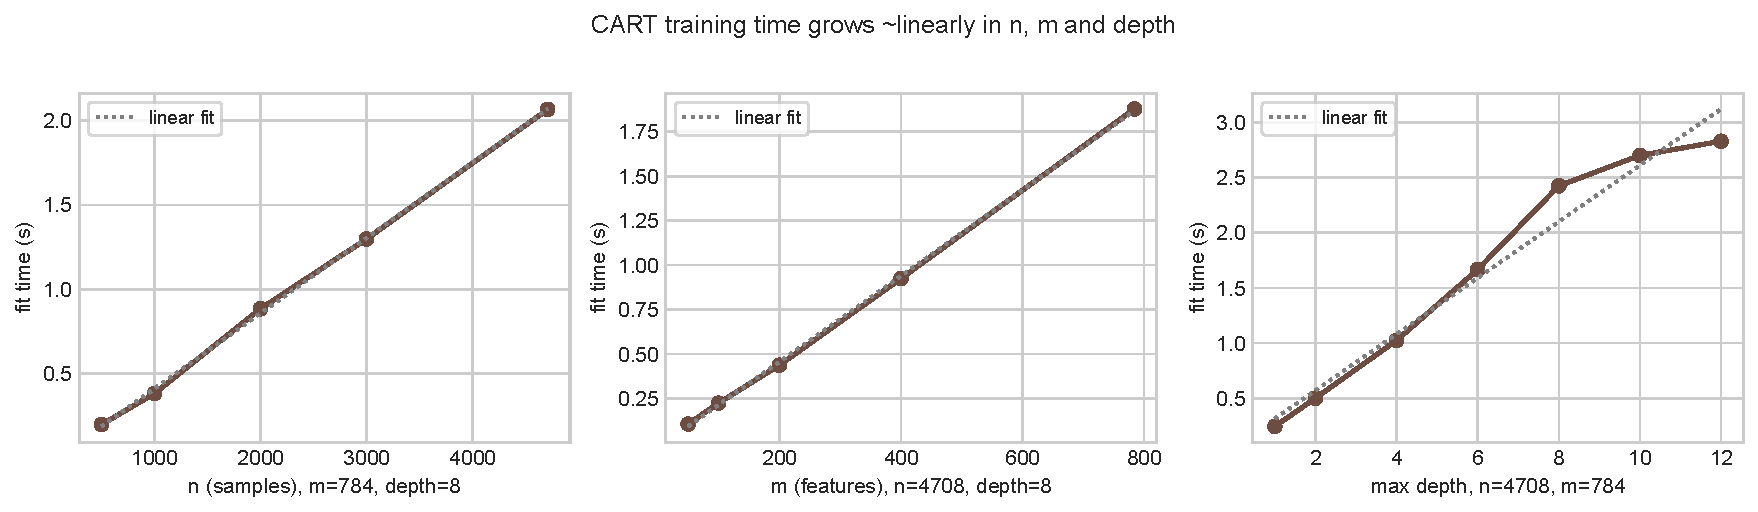
\includegraphics[width=\linewidth]{fig_tree_complexity}
  \caption{Decision tree. Top: depth selection and pixel importances (mean decrease in impurity) over the mean
           radiograph. Bottom: CART fitting time grows linearly in $n$, $m$ and depth, \ie $O(n\cdot m\cdot\text{depth})$
           up to a logarithmic factor.}
  \label{fig:tree}
\end{figure}

\begin{figure}[h]
  \centering
  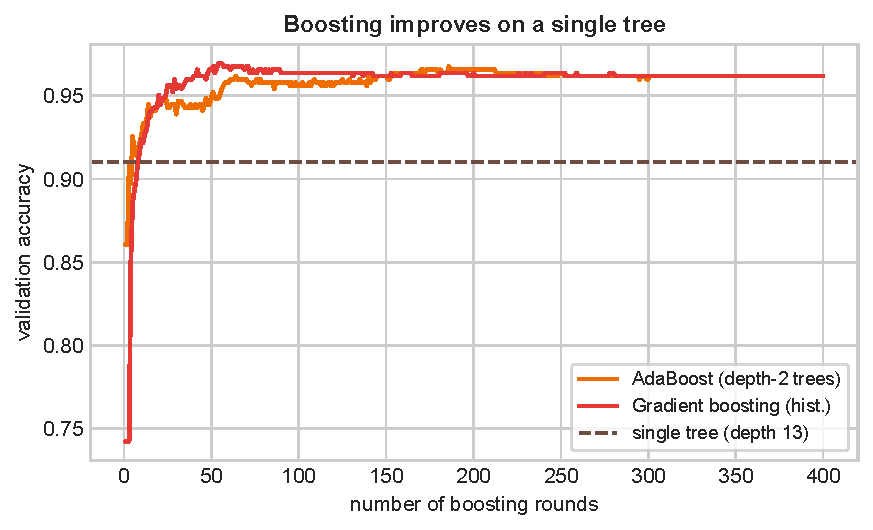
\includegraphics[width=0.6\linewidth]{fig_boosting}
  \caption{Validation accuracy against the number of boosting rounds.}
  \label{fig:boosting}
\end{figure}

\begin{figure}[h]
  \centering
  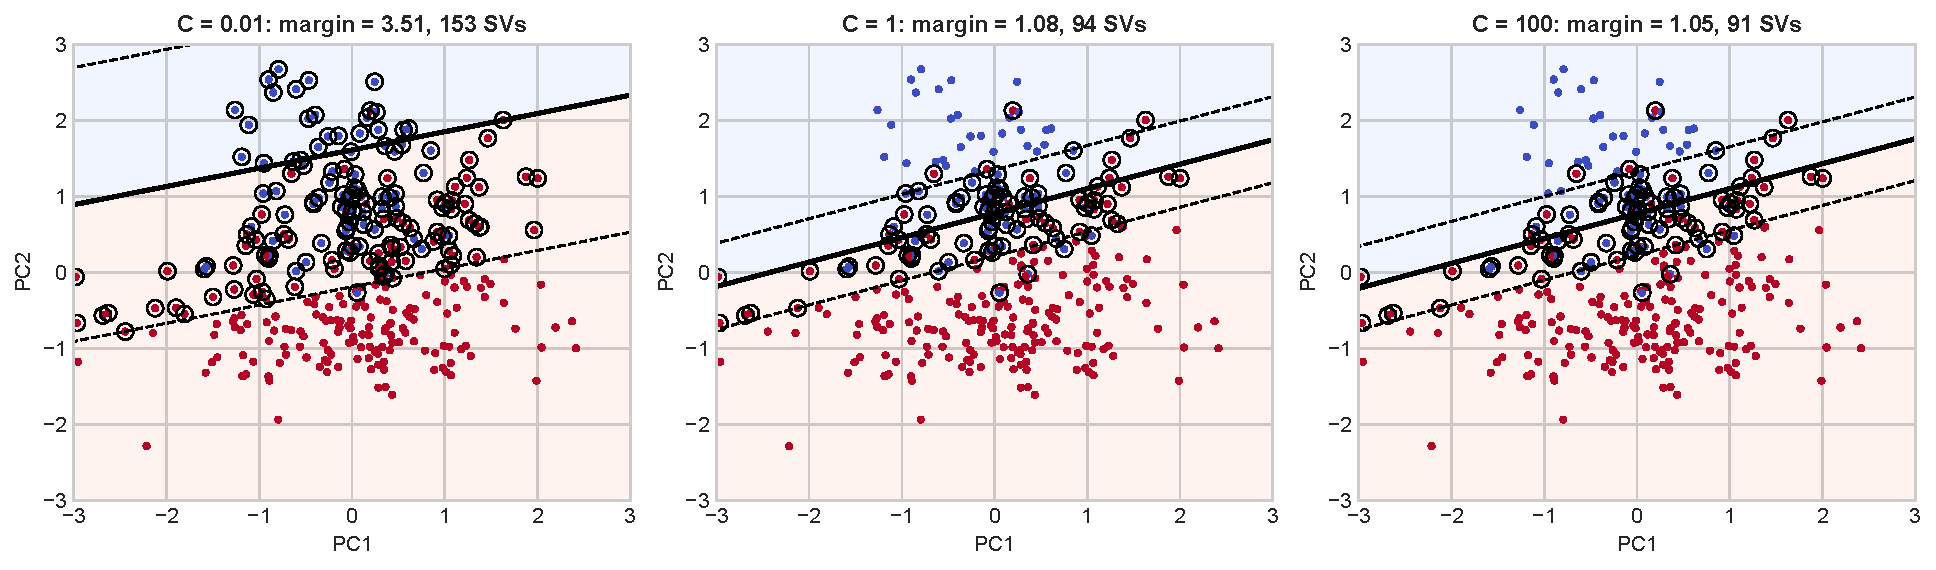
\includegraphics[width=\linewidth]{fig_svm_margin}\\[4pt]
  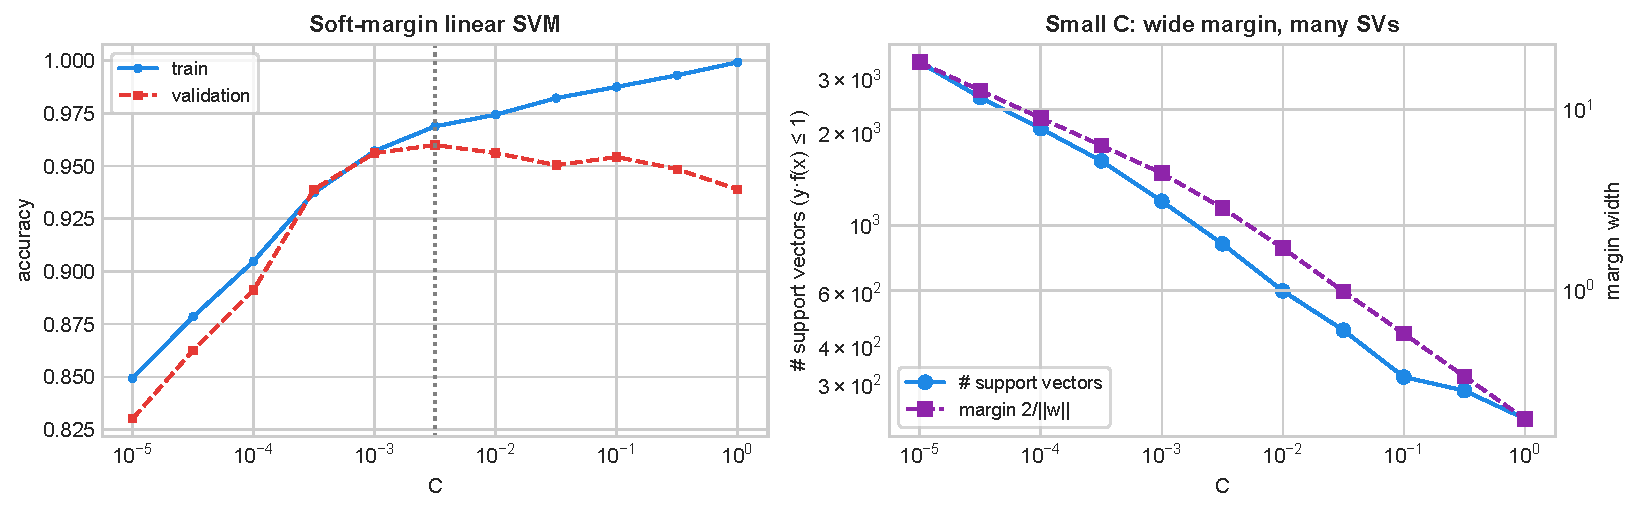
\includegraphics[width=\linewidth]{fig_svm_C}
  \caption{Support vector machines. Top: linear SVM on a 2-D projection for three values of $C$ (circled points are
           support vectors, dashed lines the margin). Bottom: on the 784 pixels, a small $C$ yields a wide margin and many
           support vectors (strong regularisation), a large $C$ a narrow margin that fits the training set.}
  \label{fig:svm}
\end{figure}

\begin{figure}[h]
  \centering
  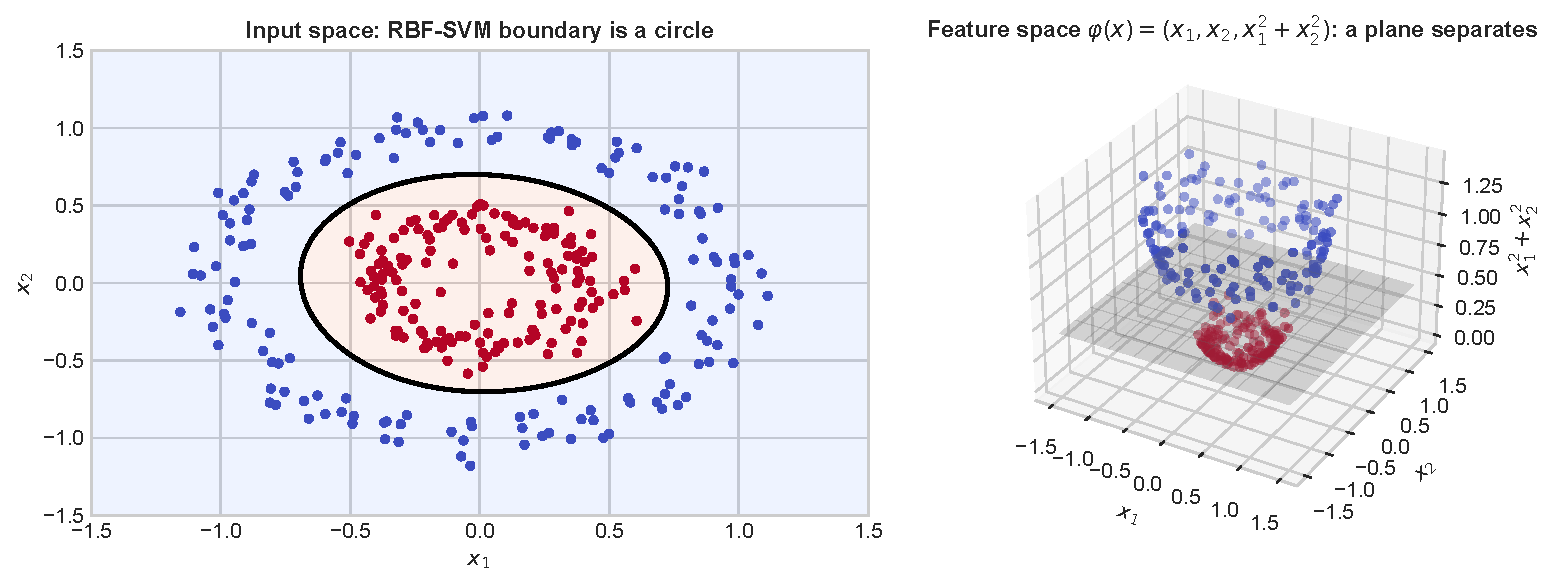
\includegraphics[width=0.62\linewidth]{fig_kernel_trick}\hfill
  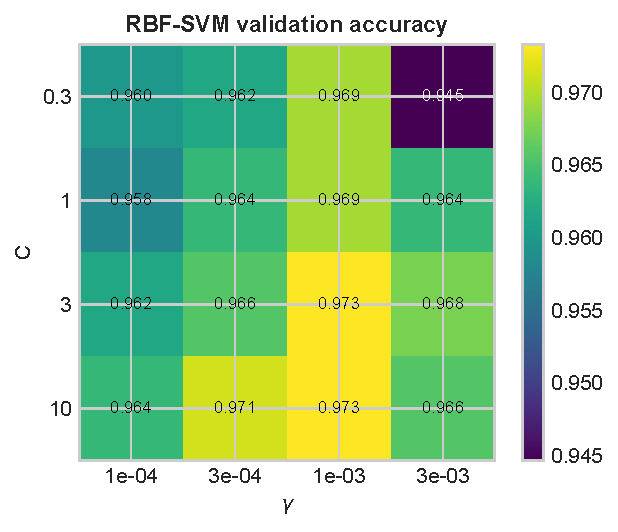
\includegraphics[width=0.34\linewidth]{fig_svm_rbf_grid}
  \caption{Left: the kernel trick, where concentric classes become linearly separable after the explicit map
           $\varphi(x)=(x_1,x_2,x_1^2+x_2^2)$; the RBF kernel does this implicitly in an infinite-dimensional space.
           Right: validation accuracy of the RBF-SVM over $(C,\gamma)$.}
  \label{fig:kernel}
\end{figure}

\begin{figure}[h]
  \centering
  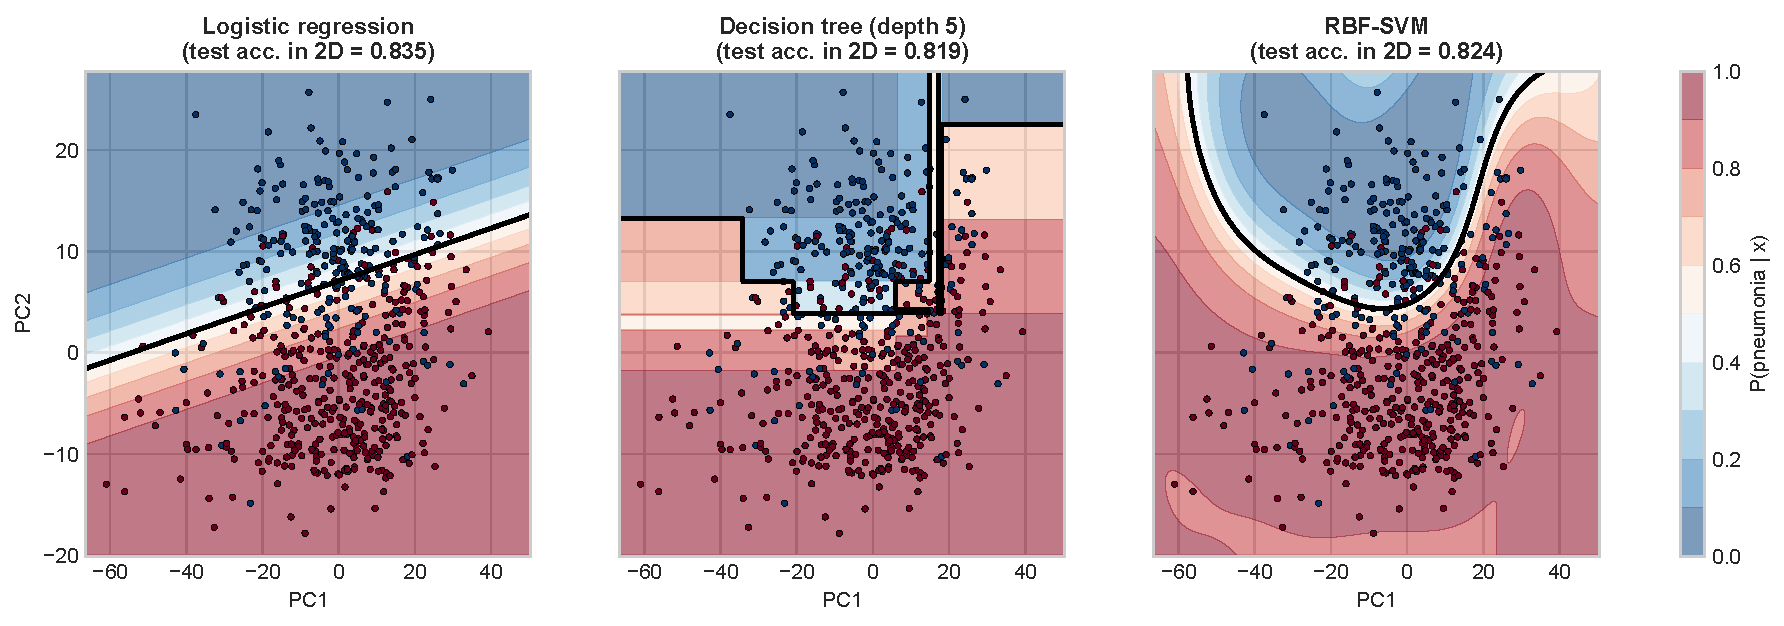
\includegraphics[width=\linewidth]{fig_boundaries}
  \caption{Decision boundaries ($P=0.5$, black) and predicted probabilities on the first two principal components:
           logistic regression (linear), decision tree (axis-aligned, piecewise constant) and RBF-SVM (smooth, curved).}
  \label{fig:boundaries}
\end{figure}

\end{document}
